\mychapter{0}{KATA PENGANTAR}
%   \begin{figure}[h]
%     \centering
%     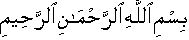
\includegraphics[width=0.5\linewidth]{images/bab0/gambarBismillah}
%   \end{figure}
  Puji Syukur kepada Tuhan yang Maha Esa, atas berkatNya penulis dapat menyelesaikan buku berjudul \textbf{\judul}. Dalam pengerjaan Tugas Akhir ini, penulis belajar banyak untuk memperdalam dan meningkatkan apa yang telah dipelajari penulis selama kuliah di Teknik Informatika ITS.
  Tugas Akhir ini terselesaikan tidak lepas dari bantuan dan dukungan banyak pihak. Oleh karena itu, pada kesempatan ini penulis mengucapkan banyak terima kasih kepada:
  \begin{enumerate}
  	\item \textbf{Daddy Jesus} - atas segala berkat, karunia, kesempatan dan rancangan jalanNya-lah penulis masih diberi nafas kehidupan, tenaga dan daya pikir untuk menyelesaikan buku ini. \textit{Thank you, Big Daddy.}
    \item \textbf{Papa dan Mama} yang selalu menguatkan, menasehati, dan luar biasa sabar dalam mengingatkan penulis agar tidak lupa menjaga kesehatan dan tidak lupa ke gereja selama masa studi.
    \item \textbf{Yth. Bapak Rully Soelaiman} yang memberi inspirasi kepada penulis untuk berpikir \textit{scientifically}, bimbingan, nasehat, saran dan memberikan penulis sisi pemikiran dan perspektif baru terhadap setiap masalah.
    \item \textbf{Yth. Bapak Rizky Januar Akbar} sebagai dosen pembimbing yang memberi bimbingan, saran teknis dan administratif, diskusi dan pemecahan masalah dalam pembuatan dan penulisan buku tugas akhir.
    \item \textbf{Keluarga XL Future Leader Scholarship Camp Batch 5} dan KSE ITS yang telah memberikan penulis kesadaran, semangat dan inspirasi untuk terus melanjutkan tugas akhir di saat penulis kehilangan semangat.
    \item \textbf{Keluarga Admin Lab. Pemrograman }(2014 - 2017) , yang telah memberikan penulis banyak pengalaman, pengetahuan dan cerita-cerita untuk dikenang.
    \item \textbf{Keluarga Alumni Budi Mulia Siantar-Surabaya angkatan 2013 } , teman setia disaat suka maupun duka.
    \item  \textbf{Keluarga Pengpro \textit{Furions} dan HMTC Optimasi 2016 }, yang mengajarkan penulis tentang cara organisasi, cara berbicara di depan publik, dan banyak lagi.    
    \item Serta semua pihak yang tidak tertulis - yang telah turut membantu penulis dalam menyelesaikan Tugas Akhir ini.
  \end{enumerate}
  Penulis menyadari bahwa Tugas Akhir ini masih memiliki banyak kekurangan. Oleh karena itu, penulis berharap kritik dan saran dari pembaca sekalian untuk memperbaiki buku ini ke depannya.


  \hfill Surabaya, Juni 2017 \\ \\ 


  \hfill Ronauli Silva N. Sidabukke

\cleardoublepage % Mengisi penanda halaman genap yang kosong

